
\documentclass[tikz]{standalone}
\usepackage{graphicx}
\usepackage{lmodern}
\usepackage{amsmath, amssymb, amsfonts}
\usetikzlibrary{calc}
\newcommand{\R}{\mathcal{R}}

\begin{document}

%abstain alpha = 1/2
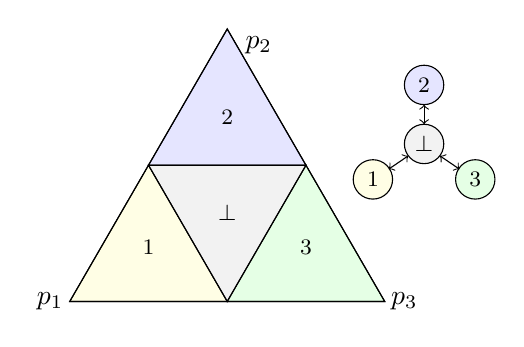
\begin{tikzpicture}
\draw (2,0) -- (-2,0) -- (0,3.46) -- cycle;
%label outcomes
\node at (-9/4, 0) {$p_1$};
\node at (2/5, 3.25) {$p_2$};
\node at (9/4, 0) {$p_3$};
%level sets
\draw[fill = blue, fill opacity = 0.1] (-1, 1.73) -- (1, 1.73) -- (0, 3.46) -- cycle; \node at (0, 1.73*1.35) {\footnotesize$2$};
\draw[fill = green, fill opacity = 0.1] (2,0) -- (1, 1.73) -- (0,0) -- cycle;
\node at (1, 1.73*0.4) {\footnotesize$3$};
\draw[fill = yellow, fill opacity = 0.1] (-2,0) -- (-1, 1.73) -- (0,0) -- cycle;
\node at (-1, 1.73*0.4) {\footnotesize$1$};
\draw[fill = gray, fill opacity = 0.1] (1,1.73) -- (-1, 1.73) -- (0,0) -- cycle;
\node at (0, 1.73*0.65) {\footnotesize$\bot$};

\draw [fill = gray, fill opacity = 0.1] (2.5, 2) circle (0.25);
\draw [fill = blue, fill opacity = 0.1] (2.5, 2.75) circle (0.25);
\draw [fill = yellow, fill opacity = 0.1] (1.85, 1.55) circle (0.25);
\draw [fill = green, fill opacity = 0.1] (3.15, 1.55) circle (0.25);
\draw[<->] (2.5, 2.25) -- (2.5, 2.5);
\draw[<->] (2.3, 1.85) -- (2.05, 1.68);
\draw[<->] (2.7, 1.85) -- (2.95, 1.68);

\node at (2.5,2) {\footnotesize$\bot$};
\node at (2.5,2.75) {\footnotesize$2$};
\node at (1.85,1.55) {\footnotesize$1$};
\node at (3.15, 1.55) {\footnotesize$3$};
\end{tikzpicture}

%%abstain alpha = 1/2 with normals
%\begin{tikzpicture}
%\draw (2,0) -- (-2,0) -- (0,3.46) -- cycle;
%%label outcomes
%\node at (-9/4, 0) {$p_1$};
%\node at (2/5, 3.25) {$p_2$};
%\node at (9/4, 0) {$p_3$};
%%level sets
%\draw[fill = blue, fill opacity = 0.1] (-1, 1.73) -- (1, 1.73) -- (0, 3.46) -- cycle; \node at (0, 1.73*1.35) {\footnotesize$2$};
%\draw[fill = green, fill opacity = 0.1] (2,0) -- (1, 1.73) -- (0,0) -- cycle;
%\node at (1, 1.73*0.4) {\footnotesize$3$};
%\draw[fill = yellow, fill opacity = 0.1] (-2,0) -- (-1, 1.73) -- (0,0) -- cycle;
%\node at (-1, 1.73*0.4) {\footnotesize$1$};
%\node at (0, 1.73*0.65) {\footnotesize$\bot$};
%
%%normals
%\draw[->] (-1/2, 1.73/2) -- (-.26, 1.0904);
%\node at (-0.45, 1.1) {\footnotesize$v_1$};
%\draw[->] (0, 1.73) -- (0, 1.73 * 0.8);
%\node at (1/4, 1.73 * 0.87) {\footnotesize$v_2$};
%\draw[->] (1/2, 1.73/2) -- (.26, 1.0904);
%\node at (0.47, 1.1) {\footnotesize$v_3$};
%\end{tikzpicture}




\end{document}
%%% Local Variables:
%%% mode: latex
%%% TeX-master: t
%%% End:
